\documentclass[10pt, letterpaper]{article}

% --- CONSOLIDATED FONT ARCHITECTURE: CRIMSON PRO BODY / INTER HEADERS ---
\usepackage[utf8]{inputenc}
\usepackage[T1]{fontenc}

\usepackage[section]{placeins} % Esto fuerza a que las imágenes no se salgan de su sección

% 1. Load Primary Families
\usepackage[light]{CrimsonPro}        % Serif Body Text
\usepackage[sfdefault]{inter}         % Sans-Serif (assigned to \sffamily)
\usepackage[defaultmono]{inconsolata} % Monospace for Code

% 2. Layout & Footnote Support
\usepackage[bottom]{footmisc}         % Forces footnotes to stay at the page bottom
\usepackage{titlesec}                 % Essential for header customization

% 3. Header Styling: Mapping Section Levels to Inter (Sans-Serif)
\titleformat*{\section}{\Large\bfseries\sffamily}
\titleformat*{\subsection}{\large\bfseries\sffamily}
\titleformat*{\subsubsection}{\normalsize\bfseries\sffamily}
\titleformat*{\paragraph}{\small\bfseries\sffamily}

% 4. Global Default: Ensure the body text remains Serif (Crimson Pro)
\renewcommand{\familydefault}{\rmdefault}


% --- BIBLIOGRAPHY CONFIGURATION ---
\usepackage[backend=biber, style=numeric, sorting=none]{biblatex}
\addbibresource{references.bib}

% Ensure the body text stays Serif
\renewcommand{\familydefault}{\rmdefault}

% --- MONOSPACE FONT (For Code) ---
\usepackage{inconsolata} % A cleaner mono font for your listings

% --- PAQUETES ---
% --- CHARACTER ENCODING & FONTS ---
\usepackage[utf8]{inputenc}
\usepackage[T1]{fontenc}
\usepackage{lmodern} % Ensures Computer Modern renders sharply

% --- PAGE LAYOUT ---
\usepackage{geometry}
\geometry{margin=1in}

% --- MATHEMATICS (The Rigor) ---
\usepackage{amsmath, amssymb, amsfonts, amsthm}
\usepackage{mathtools} % For advanced math alignment

% --- TABLES (The Data) ---
\usepackage{booktabs}   % For professional horizontal rules (\toprule, etc.)
\usepackage{tabularx}   % For auto-wrapping tables
\usepackage{array}      % For custom column types
\usepackage{multirow}   % For merging rows in tables

% --- GRAPHICS & COLOR ---
\usepackage{graphicx}
\usepackage{xcolor}
\usepackage{float}      % Allows using [H] to force image placement
\usepackage{caption}
\usepackage{subcaption} % For side-by-side images

\usepackage{parskip}
\usepackage{subcaption}

% --- CODE SNIPPETS (The Engineering) ---
\usepackage{listings}
\lstset{
    basicstyle=\ttfamily\small,
    breaklines=true,
    backgroundcolor=\color{gray!10},
    frame=single,
    captionpos=b,
    commentstyle=\color{green!40!black},
    keywordstyle=\color{blue}
}

% --- LINKS & REFERENCES ---
\usepackage[colorlinks=true, linkcolor=blue, urlcolor=blue, citecolor=blue]{hyperref}

% --- LISTS & DESCRIPTIONS ---
\usepackage{enumitem}   % For controlling spacing in lists and descriptions

% --- MISC TOOLS ---
\usepackage{csquotes}   % For professional quotation marks
\usepackage{microtype}  % Improves typography (kerning and spacing)
\usepackage{underscore} % To help with underscores in text (though \_ is safer)
\usepackage{tikz}
% --- PROJECT SPECIFIC COMMANDS ---
\newcommand{\wip}[1]{\textcolor{red}{\textbf{[PENDING UPDATE]} #1}}

\usepackage{pgfplots}
\pgfplotsset{compat=1.18}
\usepgfplotslibrary{groupplots}

\usepackage{tikz}
\usetikzlibrary{shapes.geometric, arrows.meta, positioning, shadows}


\usepackage[most]{tcolorbox}


% --- FULL-WIDTH SYMMETRICAL PHASE PORTADA (V5 - Hybrid Typography) ---
\newcommand{\phaseportada}[6]{
    \newpage
    \thispagestyle{empty}
    \newgeometry{left=0cm, right=0cm, top=0cm, bottom=0cm}
    
    \begin{tcolorbox}[
        enhanced, sharp corners, boxrule=0pt,
        colframe=white, colback=white,
        width=\paperwidth, height=\paperheight,
        valign=center, left=3.5cm, right=3.5cm
    ]
        % Top Bold Line
        {\color{gray!80}\hrule height 2pt}
        
        \vspace{1.2cm}
        \begin{center}
            {\sffamily\fontsize{25}{30}\selectfont \textbf{#1}} \\ % Arg 1: Phase ID
            \vspace{0.6cm}
            {\sffamily\fontsize{25}{30}\selectfont #2}           % Arg 2: Phase Title
        \end{center}
        \vspace{1.2cm}
        
        % Bottom Bold Line
        {\color{gray!80}\hrule height 2pt}
        
        \vspace{2.5cm}
        
        % Vertical Summary Block (Hybrid Fonts)
        \noindent
        \begin{tabularx}{\linewidth}{@{} >{\sffamily\bfseries}l >{\rmfamily}X @{}}
            Tech Stack: & #3 \\ \addlinespace[15pt]
            Core Challenge: & #4 \\ \addlinespace[15pt]
            Key Insight: & #5 \\ \addlinespace[15pt]
            Operational Outcome: & #6 \\
        \end{tabularx}
    \end{tcolorbox}
    
    \restoregeometry
    \newpage
}



% --- CONFIGURACIÓN DE ENCABEZADOS (FANCYHDR) ---
\usepackage{fancyhdr}
\pagestyle{fancy}
\fancyhf{} % Limpia los encabezados por defecto

% Línea horizontal arriba
\renewcommand{\headrulewidth}{0.4pt} 

% Título de la sección en la parte superior derecha (en chiquito)
\fancyhead[R]{\small \textit{\nouppercase{\leftmark}}}

% Número de página en la parte inferior derecha
\fancyfoot[R]{\thepage}

% Ajuste para que la primera página de cada sección también tenga el encabezado
\fancypagestyle{plain}{
  \fancyhf{}
  \fancyhead[R]{\small \textit{\nouppercase{\leftmark}}}
  \fancyfoot[R]{\thepage}
  \renewcommand{\headrulewidth}{0pt}
}


\setcounter{secnumdepth}{0} % 0 turns off numbers for sections, subsections, etc.



% --- METADATOS ---
\title{
    \textbf{Sequential Decision Science \& Generative Policy Modeling in the Ride-Hailing Marketplace of Mexico City}\\[0.5cm] % \\[0.5cm] adds space before the next line
    \large Executive Briefing: Project Pienza
    \vspace*{2cm} % Forces 2cm of space after the title (replaces the 4x 0.5cm)
}

\author{
    \small % Hace la letra general más pequeña
    \begin{tabular}{c @{\hspace{2cm}} c} % Centra el contenido de cada columna
        Author: & Prepared for: \\ 
        \textbf{Bernardo Lozano Wise} & \textbf{Placeholder} \\
        \footnotesize Data Scientist, Principal Investigator & \footnotesize Placeholder \\
    \end{tabular}
    \vspace*{1cm} % Forces 1cm of space after the author block (replaces the 2x 0.5cm)
}

\date{ 
    April 28, 2026
}

\begin{document}

\maketitle

\begin{abstract}
\noindent This report presents the architecture of Project Pienza: a scale-invariant system designed to model, simulate, and optimize sequential decision logic within the ride-hailing marketplace of Mexico City. By leveraging 24 months of high-fidelity field telemetry from a Subject Matter Expert ($N=1$), Pienza transitions human "Ground Truth" into a production-ready AI digital twin.

\vspace{0.4cm}
\noindent The document details the iterative engineering lifecycle: from foundational causal audits and topological geo-remediation to the deployment of Hierarchical Policy Clones. The framework culminates in the synthesis of a scale-invariant Manifold via Conditional Generative Adversarial Networks (cGANs) and the implementation of $O(1)$ Neural Inference. By deriving an internal mobility tensor, the project establishes a production-ready environment for the autonomous simulation of stochastic urban games and provides the mathematical scaffolding required to bridge Supervised Imitation Learning from Expert Trajectories with Markov Decision Processes (MDP).

\vspace{0.4cm}
\noindent \textbf{Disclaimer:} Project \texttt{Pienza} and all associated materials, including this document and its analyses, are the product of an independent academic and research initiative. This work is intended solely for demonstration as a Data Science / Machine Learning portfolio project. All source data has undergone a multi-layered anonymization protocol to protect privacy and obfuscate proprietary information. While the models, contents and insights presented herein reflect real-world empirical outcomes, they are intended for illustrative and educational purposes and should not be used for any commercial, financial, or operational business activities.

\vspace{0.4cm}
\noindent \textbf{Keywords:} Gemini Pro API, Star Schema ERD, Idempotent ETL, SQL, Optimal Stopping Theory, Heteroscedasticity Analysis, HDBSCAN, Uber H3, Kepler.gl, El Semáforo de Palmas, XGBoost, NLP Transformers, Keras / TensorFlow, PySpark, BigQuery, NetworkX, Markov Decision Process.

\vspace{0.4cm}

\end{abstract}

\newpage
\section{Overview}

Project Pienza is a nine-month independent research initiative documenting the transition of a ride-hailing agent in Mexico City, from tactical field operations into the domain of institutional science. To digitize the agent’s experience, the research began with a high-fidelity ground-truth acquisition campaign during a strict six-week window (August 22 -- October 1, 2025).

\subsection{Initial Scope and Constraints}
The research initially attempted to predict the financial ``spread'' (the delta between upfront and realized fares). A pilot study ($N \approx 150$) established that while simple linear models outperformed initial machine learning attempts, the overall predictive power was limited by the lack of non-linear signal and the scarcity of completed trip data. Following the principle of parsimony, price variance prediction was determined to be stochastically unfeasible at this scale.

Consequently, the project's objective shifted to behavior modeling (\textbf{Multiclass Classification}). This pivot resolved the data scarcity constraint by incorporating the previously unobserved \textbf{Negative Class} (rejected offers), succesfully overcoming  \textbf{Survivorship Bias}. To maximize discriminative signal, the agent architected a set of quasi orthogonal, mutually exclusive labels designed to isolate specific rejection drivers. While capturing this strategic nuance was the primary goal, a binary classification framework (\textit{Accept vs. Reject}) was maintained as a contingency plan. By expanding the dataset to thousands of decision events, the project successfully mapped the agent's decision boundary across six distinct rejection categories and the primary accepted class (Table \ref{tab:target_census}).

\begin{table}[H]
    \centering % This centers the table on the page
    \small
    \begin{tabular}{l r r} % 'l' for left, 'r' for right (numbers align better to the right)
        \toprule
        \textbf{Primary Target Label} & \textbf{Count} & \textbf{Rate (\%)} \\
        \midrule
        \texttt{dropoff\_non\_operational} & 2,366 & 49.65 \\
        \texttt{low\_profitability} & 838 & 17.59 \\
        \texttt{long\_pickup\_time} & 366 & 7.68 \\
        \textbf{ACCEPTED (Implicit/NaN)} & \textbf{346} & \textbf{7.26} \\
        \texttt{expected\_value\_gamble} & 330 & 6.93 \\
        \texttt{dropoff\_strategic\_mismatch} & 275 & 5.77 \\
        \texttt{dropoff\_proxy} & 239 & 5.02 \\
        \texttt{system\_logic\_failure} & 5 & 0.10 \\
        \midrule
        \textbf{Total Observations} & \textbf{4,765} & \textbf{100.00} \\
        \bottomrule
    \end{tabular}
    \caption{Data Census: Distribution of the Primary Target Variable.}
    \label{tab:target_census}
\end{table}

\subsection{Data Ingestion Architecture}
To digitize the agent’s operational reality, the project utilized a dual-engine acquisition framework. \textbf{Engine 1} (GTS Webapp) captured the verified lifecycle and financial outcomes of completed missions, while \textbf{Engine 2} (OCR Pipeline) recorded the total offer stream.

The primary engine, the \textbf{Geotimestamps (GTS) Webapp}, functioned as a telemetry instrument to log, with single taps, the five critical state transitions of a mission while on the road (Table \ref{tab:lifecycle}).

\begin{table}[H]
    \centering
    \small
    \begin{tabular}{l l}
        \toprule
        \textbf{State} & \textbf{Operational Description} \\
        \midrule
        T0 & Idle; actively seeking offers. \\ \addlinespace[2pt]
        T1 & Offer accepted; transit to pickup. \textit{(Manual Upfront Fare log)} \\ \addlinespace[2pt]
        T2 & Arrived at pickup; waiting for passenger. \\ \addlinespace[2pt]
        T3 & Mission started; passenger onboard. \\ \addlinespace[2pt]
        T4 & Mission completed; transaction finalized. \textit{(Manual Realized Fare log)} \\
        \bottomrule
    \end{tabular}
    \caption{Mission Lifecycle Mapping ($T_0 \to T_4$).}
    \label{tab:lifecycle}
\end{table}

To isolate the decision boundary, a second engine utilized a custom Optical State Archival pipeline. Using an iOS Assistive Touch macro, dubbed as a ``manual cookie'', the agent captured the total offer stream. To ensure statistical integrity, the campaign enforced zero platform filters and categorized initial data gaps, that resulted from high-risk driving maneuvers, as \textbf{Missing Completely at Random (MCAR)}, yielding a high-fidelity dataset of decision events.

Data integrity was maintained through a daily \textbf{Post-Session Reconciliation Protocol}. Image assets were processed immediately after each shift through the \textbf{Google Gemini Pro API}. Subsequently, the agent performed manual backtagging of the OCR stream to populate the \texttt{reason\_primary} target variable. Concurrently, telemetry logs were consolidated into wide-format mission dossiers to calculate session-level KPIs such as \textit{Net Spread} and \textit{Accumulated Deadhead}. Executing this labeling same-day was essential to capture operational nuance before cognitive memory decay, providing the validated foundation for subsequent relational engineering.



\subsection{The Engineering-to-Science Lifecycle}
Following the acquisition phase, the project transitioned into a two-month engineering sprint (October--November 2025). The focus was centered on architectural stabilization and stateful feature synthesis, transforming disparate spreadsheets into the \texttt{pienza.db} relational warehouse via an idempotent ETL pipeline. 

As illustrated in the Entity-Relationship Diagram (Figure \ref{fig:erd_diagram}), the architecture enforces a strict linear data lineage. This design eliminates circular references and ensures total financial and operational accountability by anchoring behavioral intent to bank-settled reality:

\begin{equation}
    \texttt{offers} \xrightarrow{1:1} \texttt{trip\_events} \xrightarrow{1:0..1} \texttt{lifetime\_trips} \xrightarrow{1:1} \texttt{activity\_earnings}
\end{equation}

\begin{figure}[H]
    \centering
    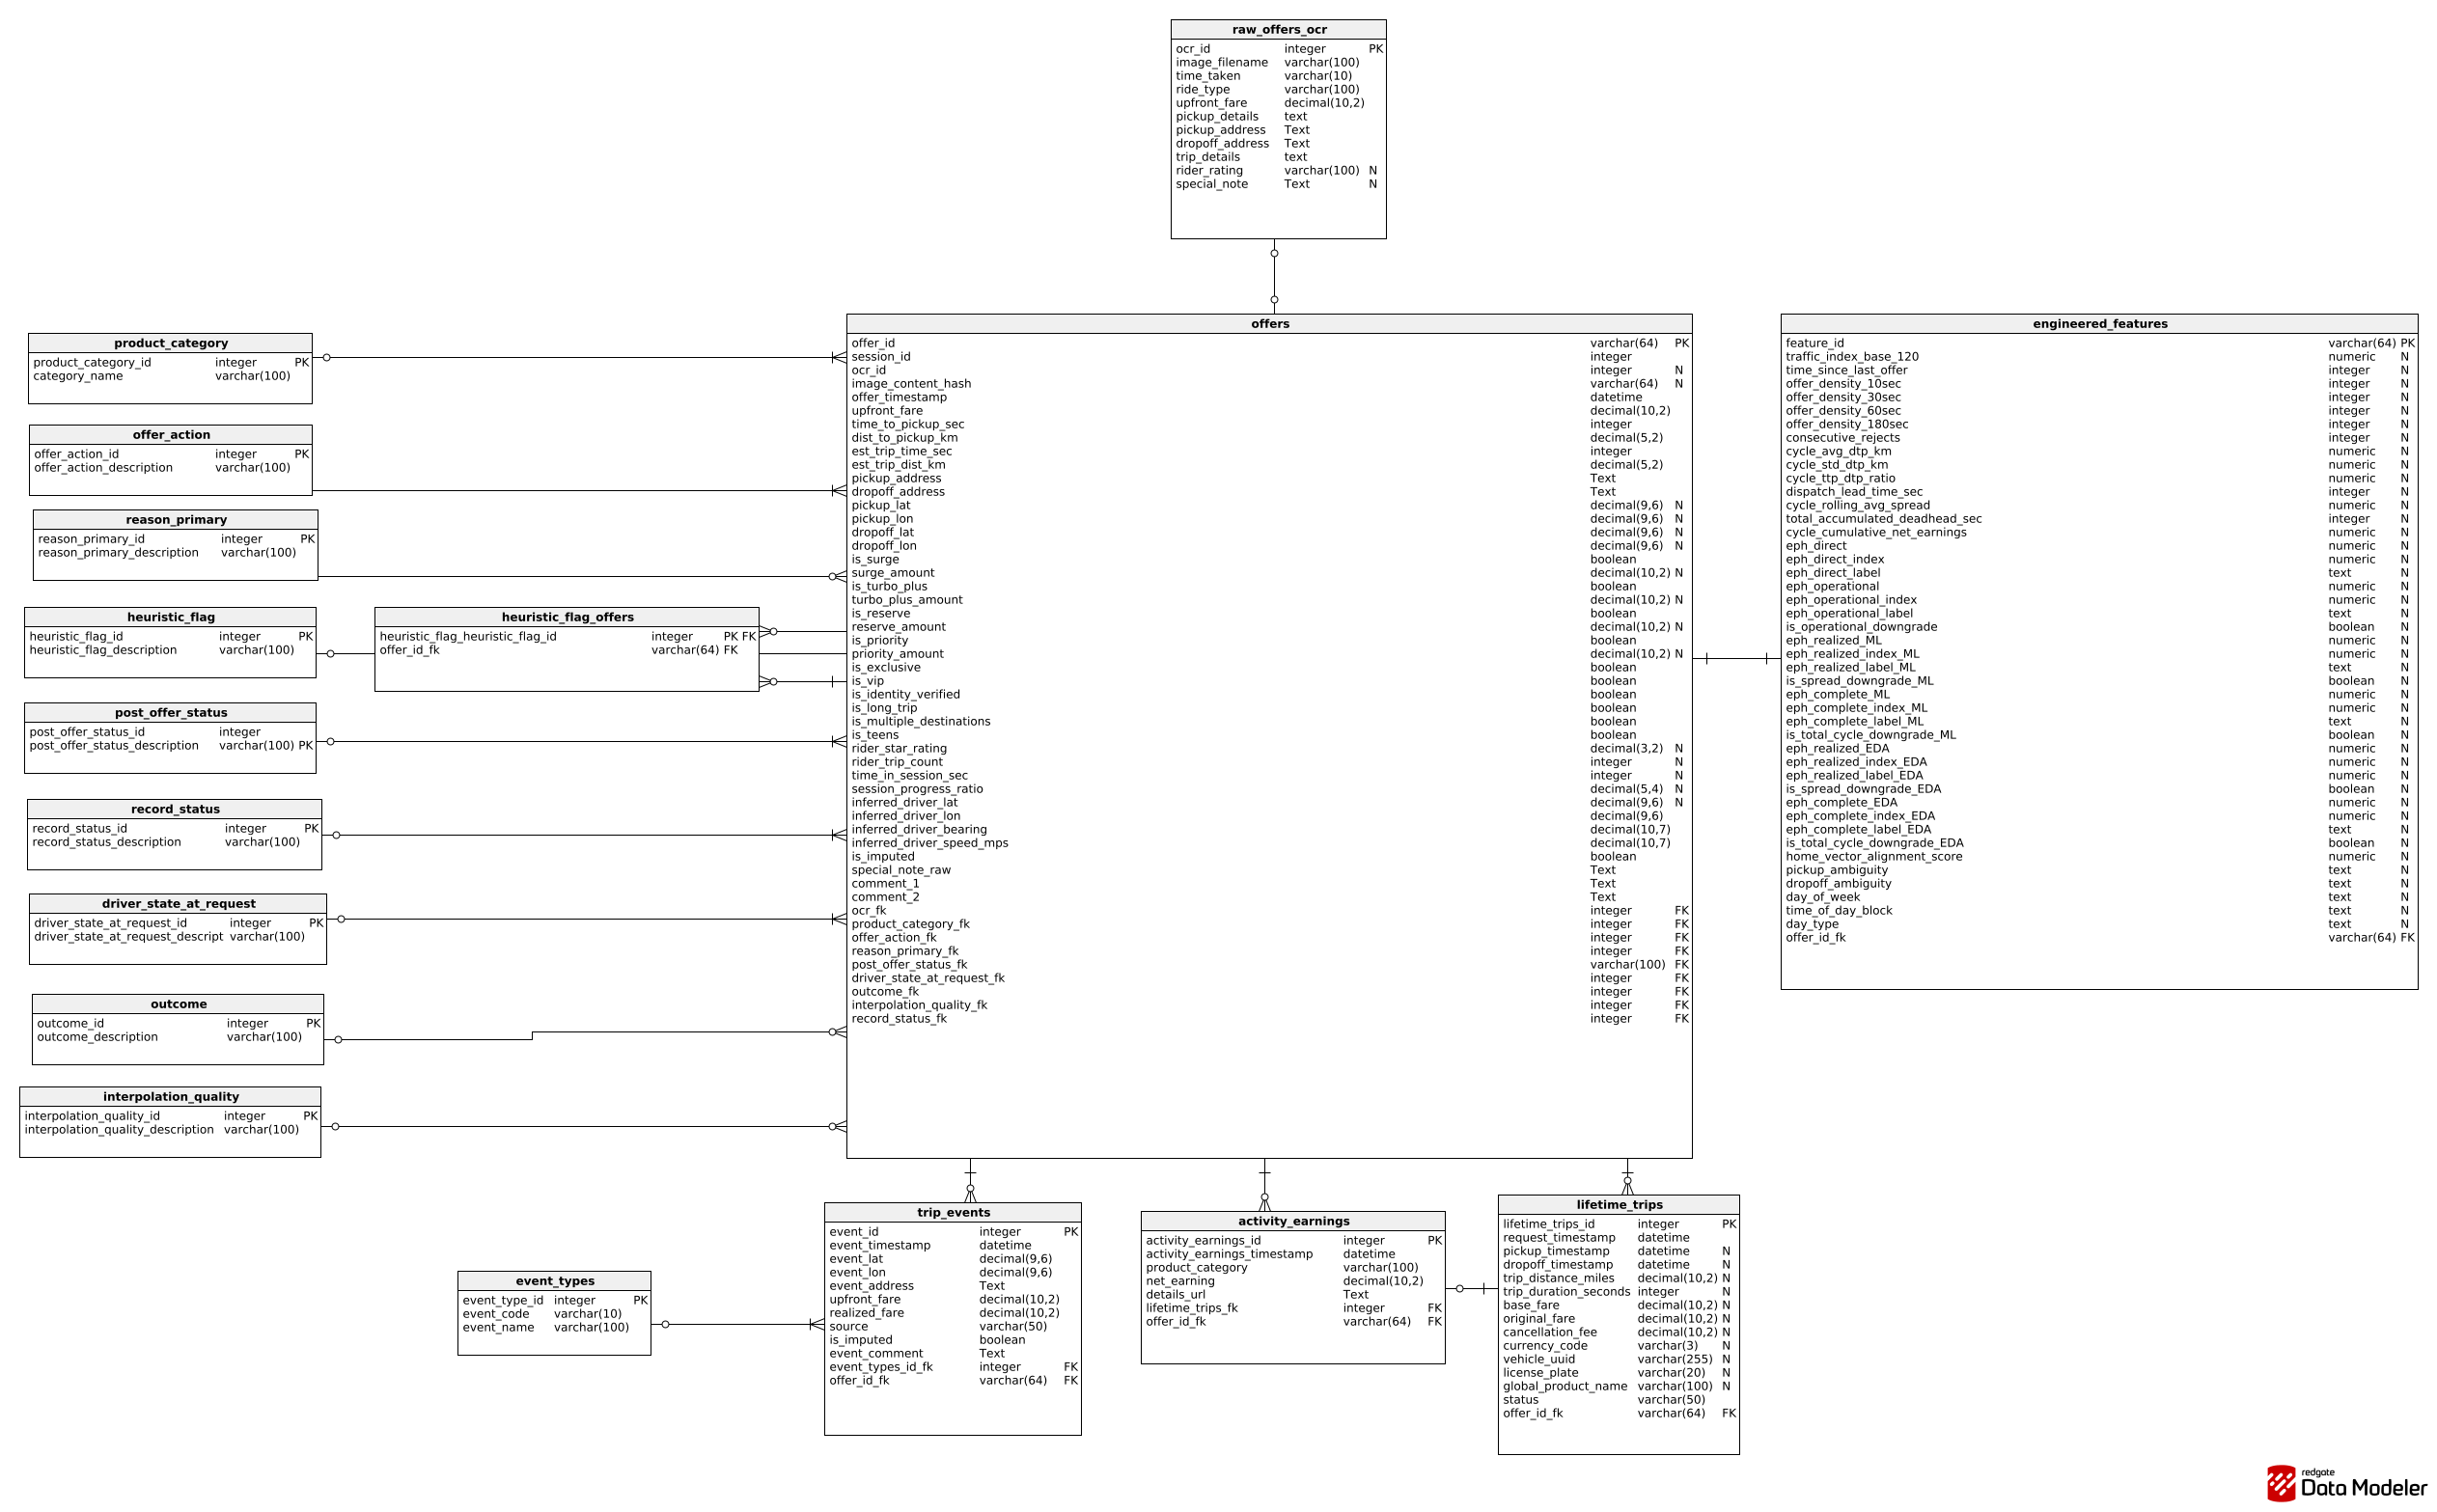
\includegraphics[width=1.0\textwidth]{Pienza_ERD.png}
    \caption{Project Pienza: Definitive Star Schema architecture. The model decouples behavioral intent (\texttt{offers}) from operational telemetry (\texttt{trip\_events}) and official platform financial ledgers.}
    \label{fig:erd_diagram}
\end{figure}

\subsection{Diagnostic Audit \& Causal Inference}

Following the relational stabilization of the dataset, a diagnostic audit was executed to deconstruct the underlying ``Economic Physics'' of the marketplace. This phase established the hard mathematical constraints and decision boundaries required for high-fidelity simulation and predictive cloning.

\begin{itemize}[leftmargin=1.5em, labelsep=0.5cm]
    \item \textbf{Search Boundary Optimization:} 
    By modeling search cycles as an \textit{Optimal Stopping Problem}, the project identified a definitive \textbf{9-minute rationality cap}. Beyond this temporal horizon, the Net Expected Value (NEV) of rejecting a viable offer in favor of a superior future event becomes negative due to the deterministic decay of accrued deadhead time.
    
    \item \textbf{Moral Hazard Mitigation:} 
    A quadratic polynomial regression was utilized to identify the tipping point where platform payouts transition from inelasticity to compensatory adjustment. The model reveals a strategic \textbf{``Integrity Buffer''} that decouples marginal labor time from marginal compensation. This architectural choice maintains price integrity for the passenger while neutralizing the incentive for intentional delay; crucially, this ensures the Agent receives full compensation for missions completed ahead of schedule,  while restricting compensatory adjustment only to exogenous shocks.
\end{itemize}


\section{Classical Machine Learning}

The star architecture of Project Pienza transitions from statistical audit to the deployment of predictive and prescriptive intelligence. This phase constructs the AI digital twin required to model high-frequency marketplace dynamics.


\subsection{Unsupervised Learning: Topology Discovery} 
Implementation of \texttt{HDBSCAN} and \texttt{K-Means} to deconstruct the city into 44 machine-discovered zones. While the initial clustering was achieved in one week, a diagnostic audit identified a systemic decoupling between raw address strings and geocoordinates. This necessitated a deep remediation campaign, spanning the terminal days of 2025, to achieve absolute parity between text syntax, spatial coordinates, and the Agent’s manually-crafted operational polygons. 

Figure \ref{pienza_hdbscan_h3_mapv3} illustrates the resulting H3-indexed hubs overlaid on the manual polygon layer.\footnote{ It is critical to note that the resulting map does not attempt to model the total ride-hailing universe of Mexico City; it is a strictly constrained mirror of the \textbf{Agent's Operational Reality}. To maintain policy fidelity, the Agent never altered his heuristics to capture exogenous data; consequently, the map reflects only the specific times and zones of the Agent's historical operations.}

\begin{figure}[H]
    \centering
    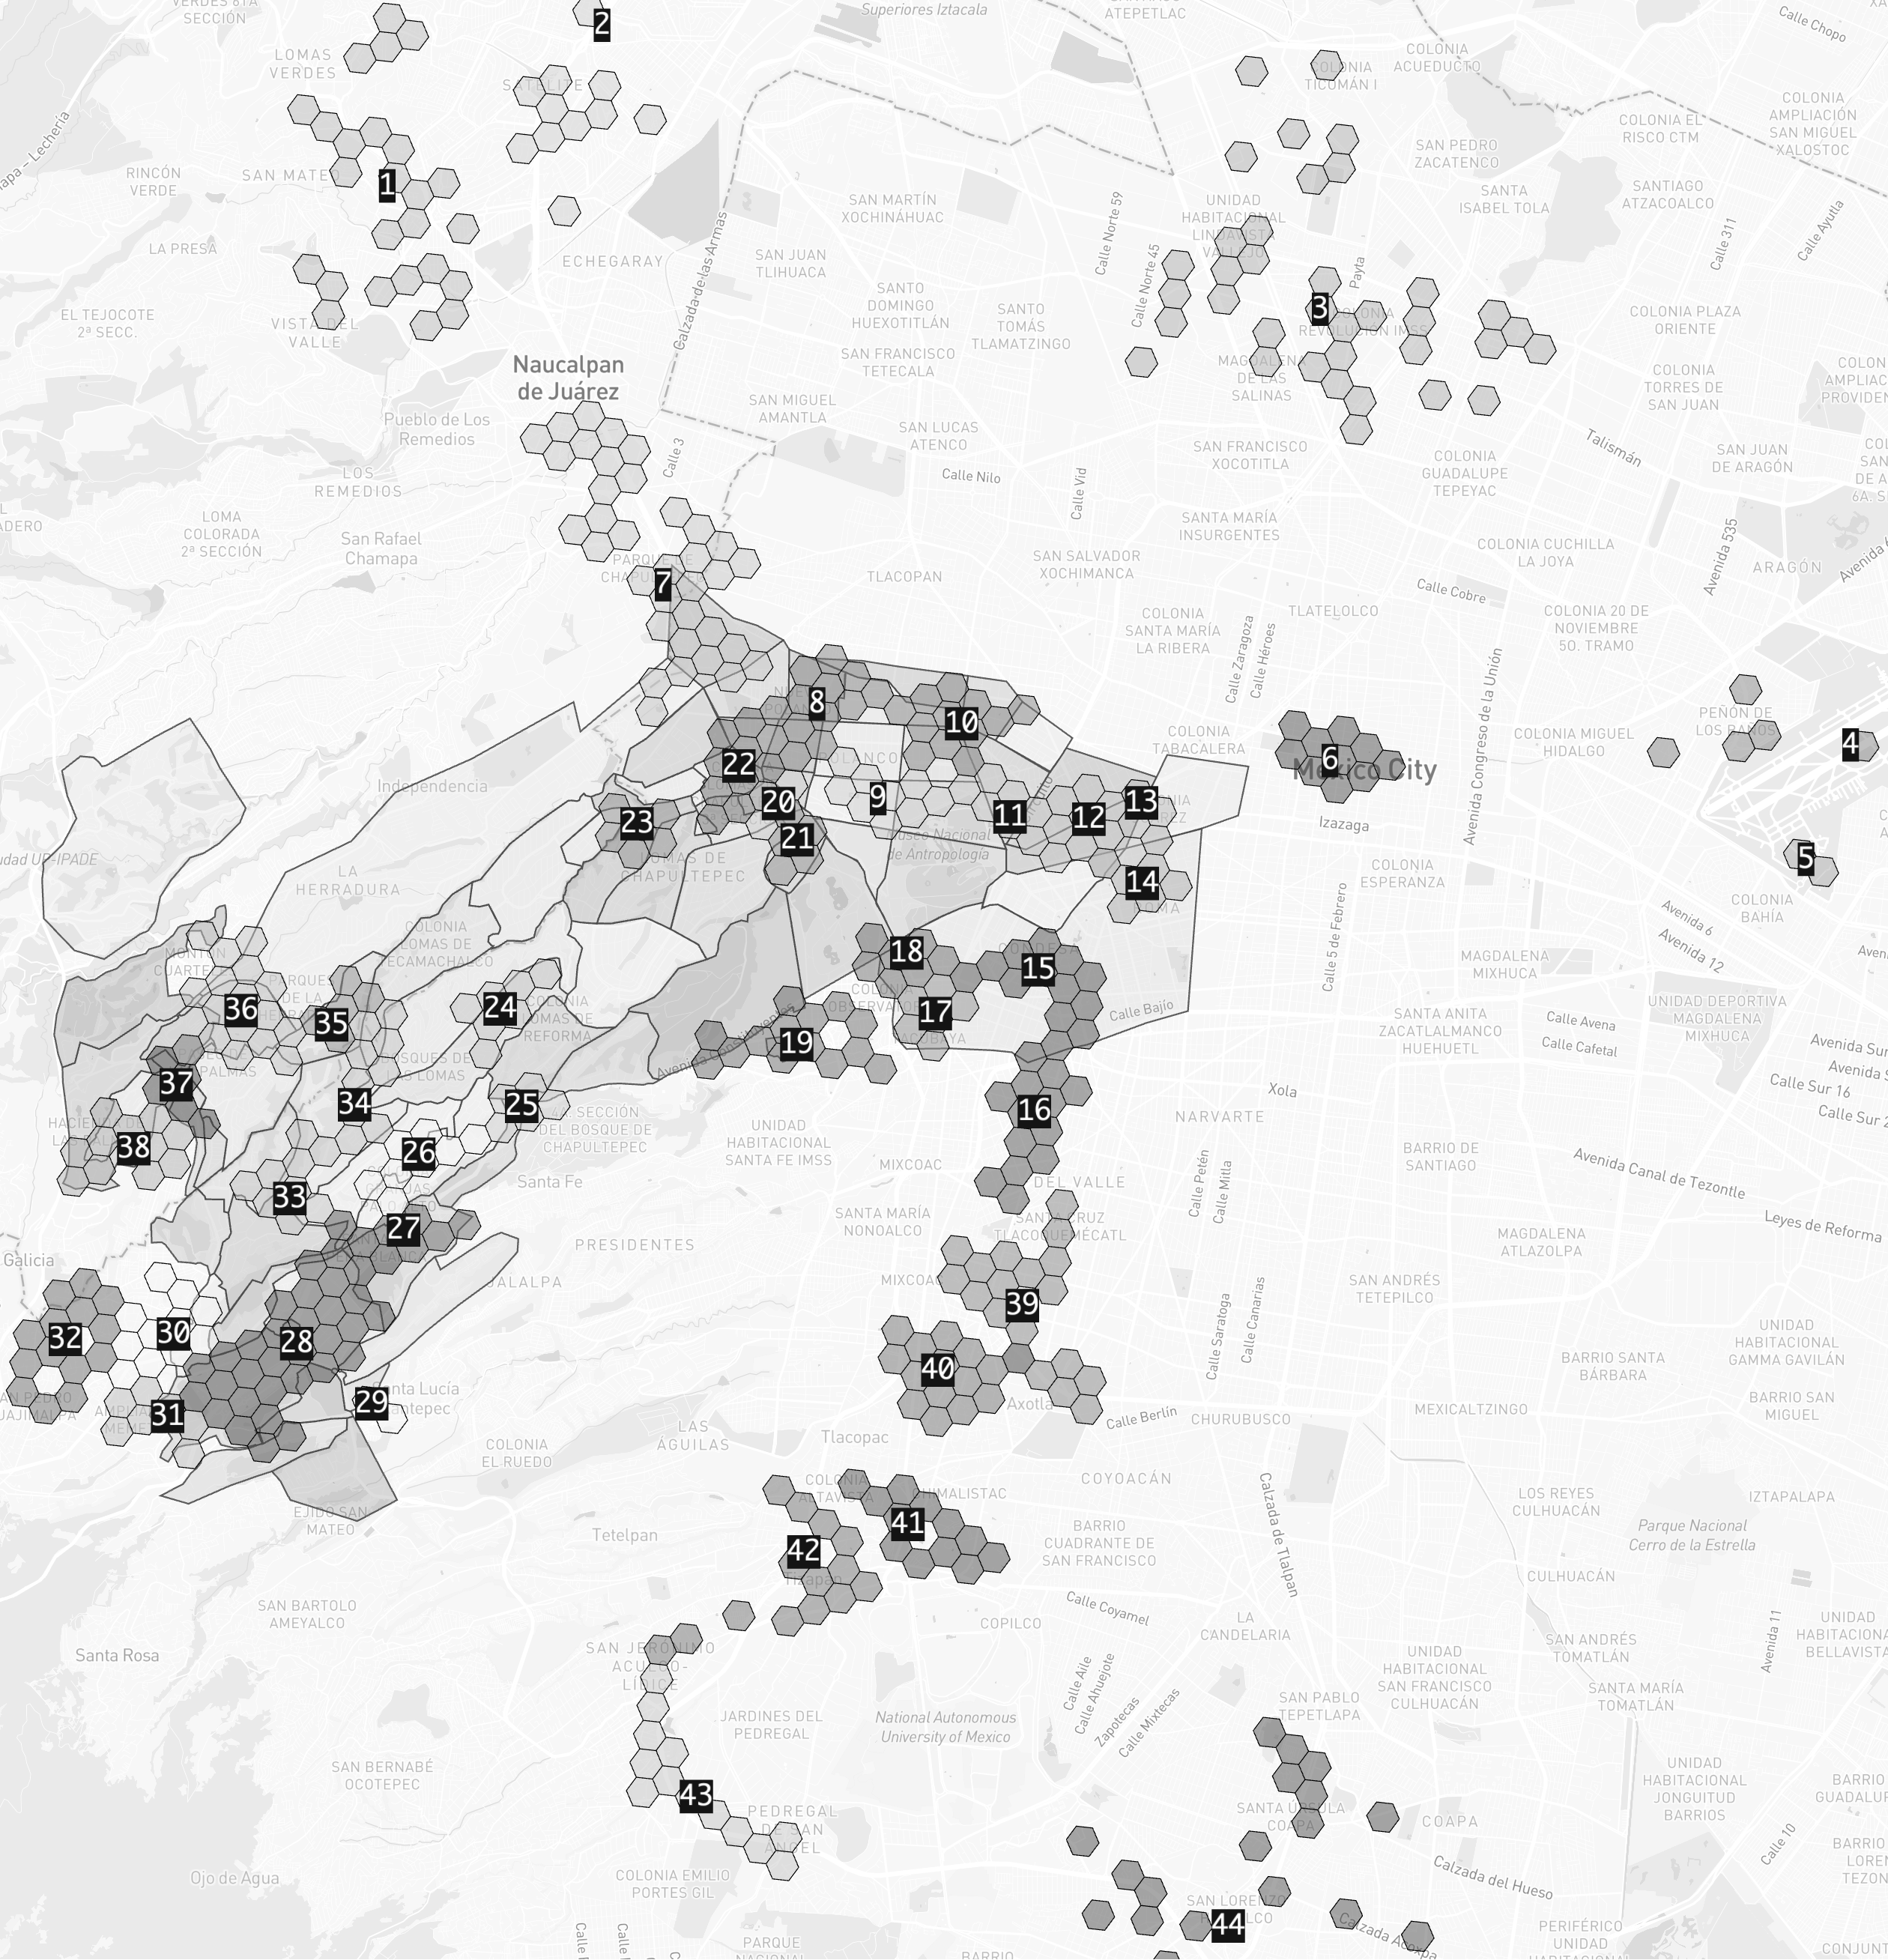
\includegraphics[width=0.92\textwidth]{pienza_hdbscan_h3_mapv3.png} 
    \caption{Topological Machine Truth: HDBSCAN clusters aggregated via H3 hexagons, revealing the organic ``Gravity Wells'' of the marketplace.}
    \label{pienza_hdbscan_h3_mapv3}
\end{figure}

\begin{table}[H]
    \centering
    \scriptsize
    \setlength{\tabcolsep}{4pt}
    \begin{tabular}{rl | rl | rl | rl}
        \toprule
        \textbf{ID} & \textbf{Hub Name} & \textbf{ID} & \textbf{Hub Name} & \textbf{ID} & \textbf{Hub Name} & \textbf{ID} & \textbf{Hub Name} \\
        \midrule
        1 & lomas\_verdes & 12 & la\_diana & 23 & cofre\_de\_perote & 34 & chamizal \\
        2 & plaza\_satélite\_mundo\_e & 13 & col\_juárez & 24 & duraznos & 35 & lomas\_anáhuac \\
        3 & central\_del\_norte & 14 & roma\_norte & 25 & tamarindos & 36 & interlomas\_magnocentro \\
        4 & terminal\_1\_aicm & 15 & condesa & 26 & nodo\_constituyentes\_reforma & 37 & vialidad\_de\_la\_barranca \\
        5 & terminal\_2\_aicm & 16 & nápoles\_wtc & 27 & santa\_fe\_patio & 38 & haciendas\_san\_fernando \\
        6 & centro\_histórico & 17 & san\_miguel\_chapultepec & 28 & santa\_fe\_core & 39 & felix\_cuevas \\
        7 & sotelo\_san\_esteban & 18 & tacubaya & 29 & santa\_fe\_itesm & 40 & barranca\_del\_muerto \\
        8 & carso\_antara\_miyana & 19 & observatorio & 30 & cruce\_echánove & 41 & san\_ángel\_altavista \\
        9 & campos\_elíseos & 20 & fc\_cuernavaca & 31 & santa\_fe\_abc & 42 & pedregal \\
        10 & polanco\_trebol & 21 & virreyes & 32 & cuajimalpa\_centro & 43 & san\_jerónimo \\
        11 & anzures\_reforma & 22 & el\_semáforo\_de\_palmas & 33 & pabellón\_bosques & 44 & viaducto\_tlalpan \\
        \bottomrule
    \end{tabular}
    \caption{Registry of the 44 machine-discovered operational hubs.}
    \label{tab:hdbscan_dictionary}
\end{table}



\subsection{Supervised Imitation Learning: From Sky to Psyche}

Initial attempts to model agent behavior utilized a flat architecture, training a single \texttt{XGBoost} classifier across the entire decision spectrum. While this model successfully learned deterministic operational boundaries (\textit{e.g., Non-Operational zones}), it failed to resolve high-order strategic nuances. The majority classes (\textit{Non-Operational, Low Profitability}) created a ``Gravitational Well,'' effectively masking the signal of the minority classes (\textit{Strategic Mismatch, Expected Value Gamble}). As a result, the flat model displayed a structural inability to isolate behavioral intent from high-volume logistical noise.

To resolve this, the architecture was decomposed into two sequential inference layers. Layer 1 acts as a \textbf{Triage Filter}, isolating deterministic noise from high-signal observations. Layer 2, the \textbf{Nuance Engine}, operates exclusively on the surviving sub-universe, allowing the model to dedicate its full predictive capacity to the subtle distinctions of strategic intent.

\subsubsection{Layer 1: The Bouncer}
Layer 1 optimizes for \textit{Recall}, ensuring that high-signal strategic events are successfully preserved for Layer 2\footnote{A 0.40 threshold was utilized as a research-specific tuning knob to maximize strategic signal recall. In production, this threshold can be dynamically recalibrated to adjust the AI twin's risk-aversion without model retraining.}.

\begin{table}[H]
    \centering
    \small
    \begin{tabular}{l c c c r}
        \toprule
        \textbf{Class Label} & \textbf{Precision} & \textbf{Recall} & \textbf{F1-Score} & \textbf{Support} \\
        \midrule
        \texttt{THE\_NUANCED\_REST} & 0.70 & 0.70 & 0.70 & 164 \\ \addlinespace[2pt]
        \texttt{long\_pickup}        & 0.50 & 0.96 & 0.66 & 56  \\ \addlinespace[2pt]
        \texttt{low\_profitability}  & 0.69 & 0.73 & 0.71 & 128 \\ \addlinespace[2pt]
        \texttt{non\_operational}     & 0.96 & 0.81 & 0.88 & 391 \\ \addlinespace[2pt]
        \texttt{dropoff\_proxy}      & 0.81 & 0.85 & 0.83 & 41  \\ \addlinespace[4pt]
        \midrule
        \textbf{Macro Average}       & \textbf{0.73} & \textbf{0.81} & \textbf{0.76} & \textbf{780} \\
        \bottomrule
    \end{tabular}
    \caption{Layer 1 Classification Report: Triage aggregates for noise filtration.}
    \label{tab:layer1_report}
\end{table}

\subsubsection{Layer 2: The Nuance Engine}
Operating on the purified output of Layer 1, the Strategist resolves the final decision classes. This architecture prevents majority-class noise from interfering with the Agent's strategic logic, resulting in a significant uplift in behavioral cloning performance.

\begin{table}[H]
    \centering
    \small
    \begin{tabular}{l c c c r}
        \toprule
        \textbf{Class Label} & \textbf{Precision} & \textbf{Recall} & \textbf{F1-Score} & \textbf{Support} \\
        \midrule
        \texttt{ACCEPTED}               & 0.92 & 0.91 & 0.92 & 67 \\ \addlinespace[2pt]
        \texttt{strategic\_mismatch}    & 0.96 & 0.95 & 0.95 & 56 \\ \addlinespace[2pt]
        \texttt{expected\_value\_gamble}& 0.84 & 0.88 & 0.86 & 41 \\ \addlinespace[4pt]
        \midrule
        \textbf{Macro Average}          & \textbf{0.91} & \textbf{0.91} & \textbf{0.91} & \textbf{164} \\
        \bottomrule
    \end{tabular}
    \caption{Layer 2 Classification Report: Strategic decision cloning performance.}
    \label{tab:layer2_report}
\end{table}


\section{Generative Moonshots}

While the \textit{Cognitive Cascade} utilized state-space awareness to capture the full operational context of each offer, the architecture remained constrained by "Snapshot Indifference"—a fundamental limitation where tabular models evaluate offers in a vacuum, failing to account for the hidden momentum of a work shift. To resolve this, the framework transitioned to deep-learning architectures to model the "Expert Rhythm," where every decision is processed as a dynamic function of the market’s state. This generative foundation establishes the definitive baseline for future \textbf{Reinforcement Learning (RL)} deployments and full-scale \textbf{Markov Chain Montecarlo (MCMC)} simulations, specifically designated as future research for "Pienza 2.0: The Knowledge in the Age of AI".

\subsection{The Quest to O(1) Inference: NLP Transformers}
In a production environment, the current architecture would rely on external geocoding APIs, constrained by high network I/O latency ($>500$ms). To bypass this, the project engineered \textbf{miniBabel}: a locally-hosted Transformer that maps raw urban syntax directly to a \texttt{zone\_id}. This architecture reduces end-to-end latency to $<10$ms, providing a bridge toward the high-availability horizon of bitwise H3 integer indexing (Table \ref{tab:babel_efficiency}).

\begin{table}[H]
    \centering
    \small
    \begin{tabularx}{\textwidth}{l l l l X}
        \toprule
        \textbf{Architecture} & \textbf{Method} & \textbf{Complexity} & \textbf{Latency} & \textbf{Strategic Value} \\
        \midrule
        External API & Geometric PiP & $O(N \times M)$ & High ($>500$ms) & Research-only; high I/O risk. \\
        \addlinespace
        \textbf{miniBabel} & \textbf{Neural Inference} & $\mathbf{O(1)}$ & \textbf{Low ($<10$ms)} & \textbf{Production-ready; autonomous.} \\
        \addlinespace
        Uber H3 & Hash Lookup & $O(1)$ (Bitwise) & Ultra-Low ($<1$ms) & Ideal target for fleet-scale telemetry. \\
        \bottomrule
    \end{tabularx}
    \caption{Comparative Efficiency: Algorithmic complexity and latency.}
    \label{tab:babel_efficiency}
\end{table}

The project benchmarked a custom-built Transformer against a state-of-the-art pre-trained baseline.
\begin{itemize}[noitemsep, topsep=3pt]
    \item \textbf{miniBabel (Custom Urban Transformer):} Restricted to two attention layers with a high-dropout bottleneck ($p=0.2$). 
    \item \textbf{miniBETO (Spanish BERT Adaptation):} Adaptation of a pre-trained Spanish BERT model. 
\end{itemize}

Performance metrics were selected to account for geographic class imbalances and operational throughput requirements.

\begin{table}[H]
    \centering
    \small
    \begin{tabular}{l c c c r}
        \toprule
        \textbf{Architecture} & \textbf{Params} & \textbf{Epochs} & \textbf{Acc.} & \textbf{Macro F1} \\
        \midrule
        Custom Transformer (\textit{miniBabel}) & $\approx 1.5$M & 22 & 83.04\% & 0.79 \\
        \addlinespace
        \textbf{BETO (Spanish BERT)} & $\approx \mathbf{110}$\textbf{M} & \textbf{17} & \textbf{86.58\%} & \textbf{0.84} \\
        \bottomrule
    \end{tabular}
    \caption{Performance metrics for the NLP urban inference tournament.}
    \label{tab:nlp_benchmarks}
\end{table}

\noindent While \textbf{BETO} achieves higher absolute performance, \textbf{miniBabel} maintains a highly competitive 0.79 F1-score with less than 2\% of the parameter count. 



\section{Synthetic Simulation \& Scalability}

To overcome the data sparsity of the initial ground-truth cohort ($N \approx 4,700$), a \textbf{Conditional Generative Adversarial Network (cGAN)} was deployed. This architecture synthesizes a 1,000,000-row data manifold conditioned on specific market states—such as \textit{Time of Day}, \textit{Product Tier}, and \textit{Operational Zone}—effectively transforming the static dataset into an infinite Keras generator of operationally-valid ride offers.

The generator operates through a four-stage dense neural funnel, mapping market constraints to continuous physical outcomes (fare, duration, and distance). To ensure statistical parity, the training pipeline implemented \textit{Log-Normal Transformations} and \textit{MinMax Scaling} to stabilize gradients and prevent mode collapse. Final validation confirmed high distributional fidelity, with a Mean Jensen-Shannon Divergence of 0.076 and a KS statistic below 0.05, proving the synthetic market physics deviate by less than 5\% from ground-truth reality.

This implementation establishes a production-ready foundation for autonomous fleet prototyping and policy stress-testing. By decoupling high-volume simulation from local file-based computation via \textbf{Google BigQuery} and \textbf{Apache Spark (PySpark)}, the framework achieves scale-invariance. The simulation engine provides the necessary mathematical scaffolding to transition from reactive decision-making to a prescriptive \textit{Markov Decision Process} (MDP), where every dispatch action is optimized to maximize future state-value.



\section{Network Graph Analysis: A Sandbox for AV's}

The project transitions from row-wise analysis to graph-based intelligence by deconstructing the city as a network rather than a collection of points. This topological assessment identifies the latent connectivity and economic gravity governing high-yield mission sequences.

% Forzamos la figura justo debajo del párrafo introductorio
\begin{figure}[H]
    \centering
    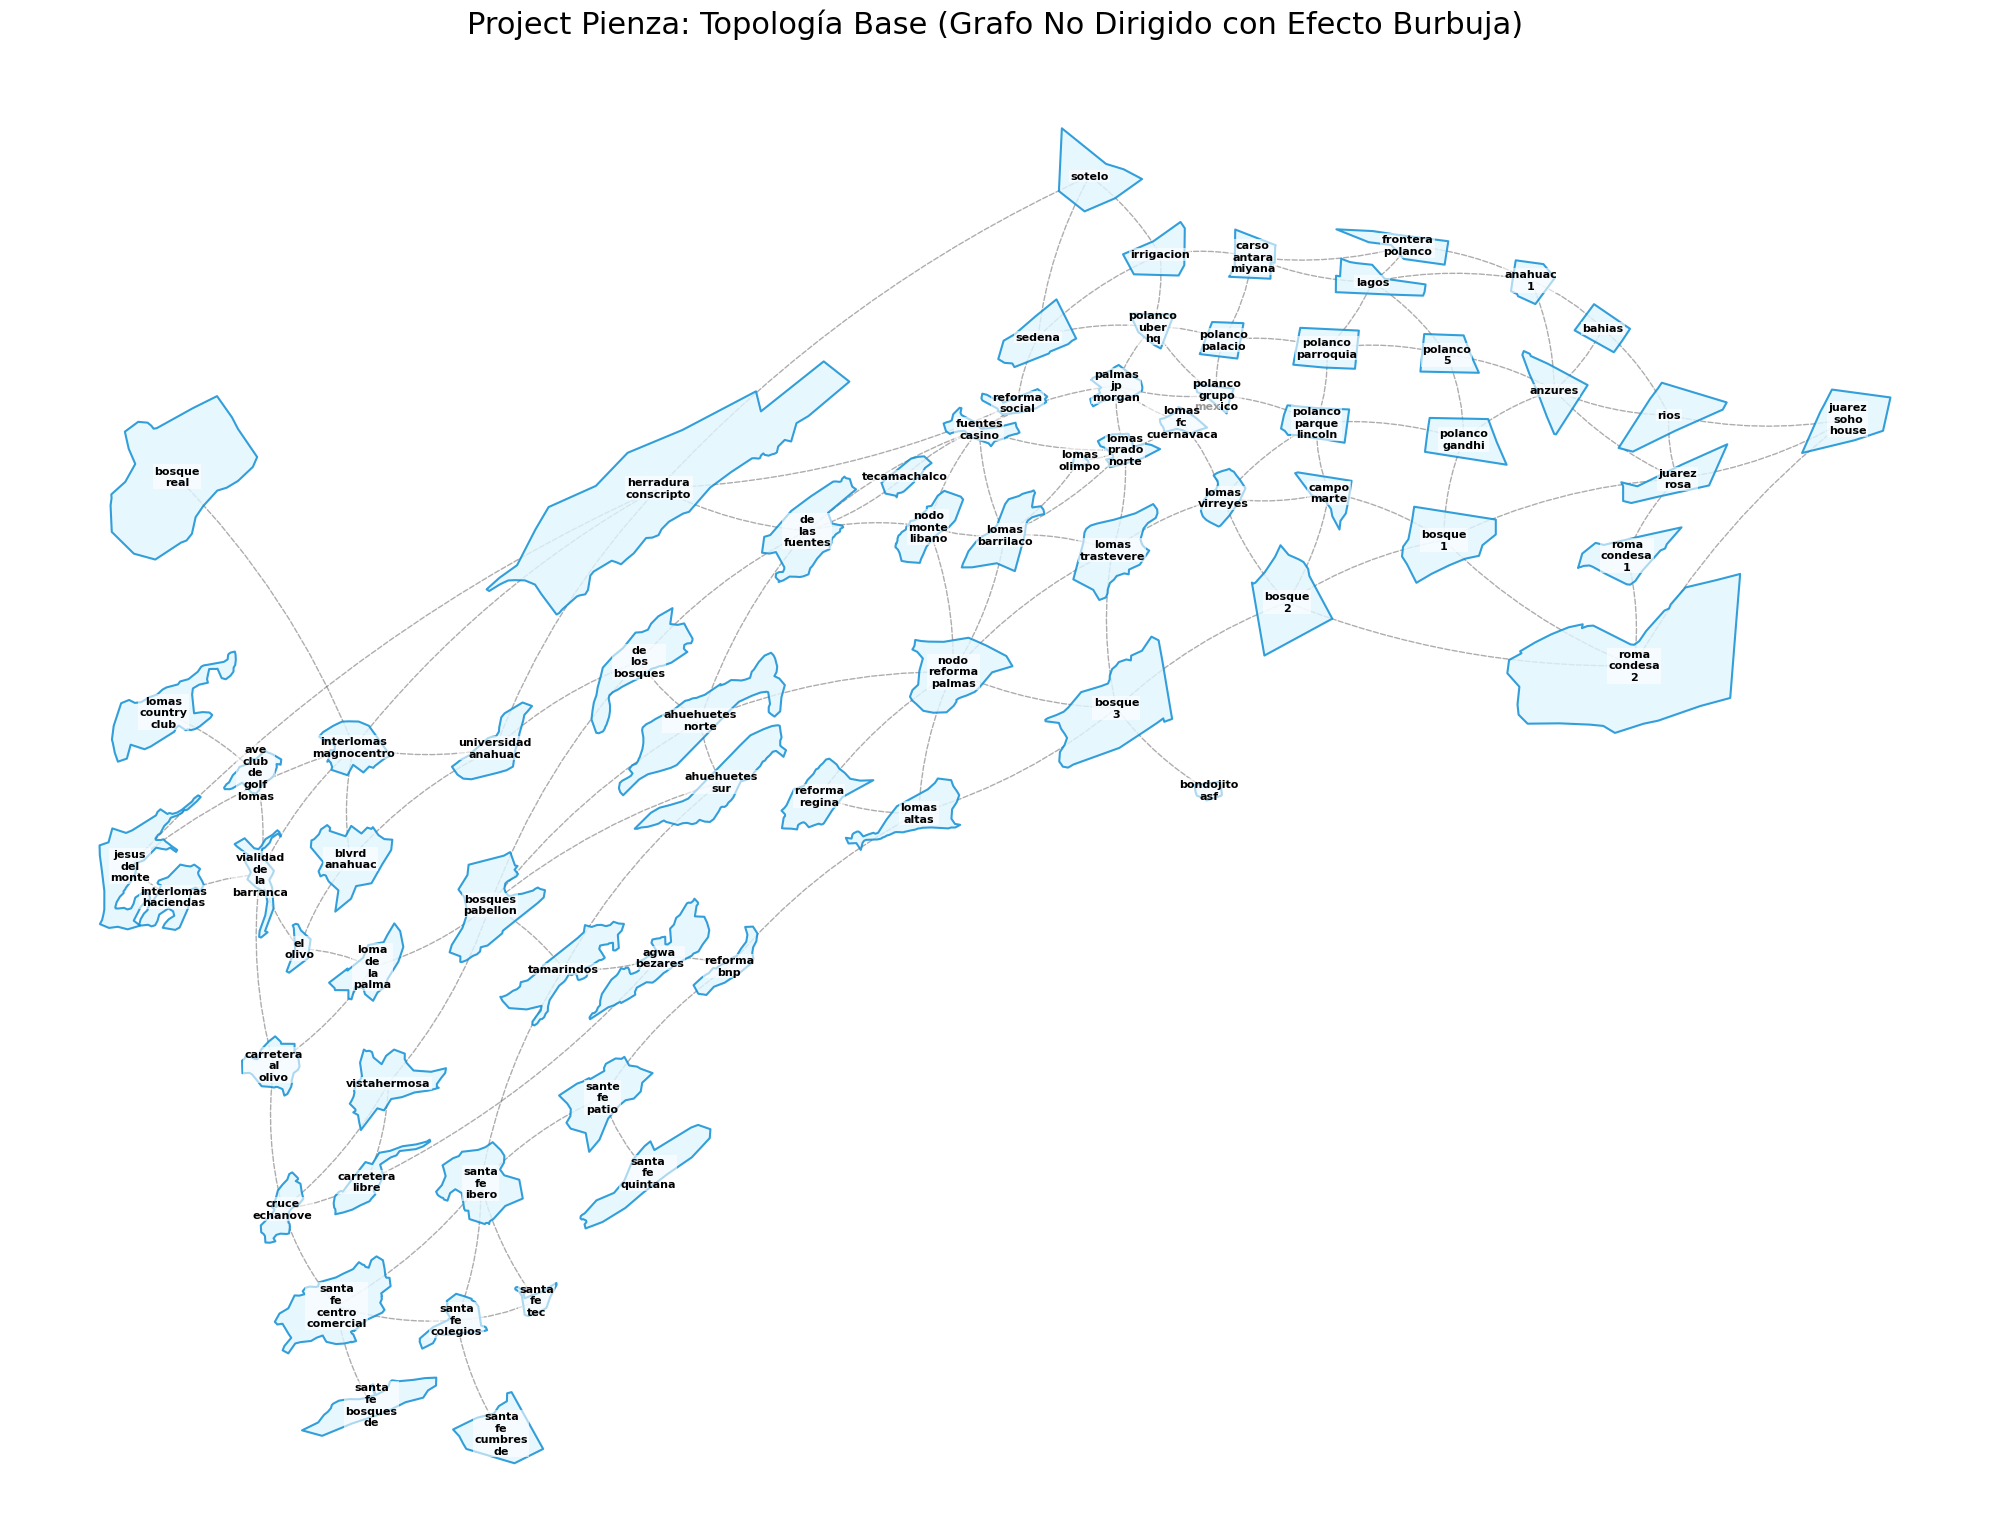
\includegraphics[width=0.85\textwidth]{fig_base_topology.png} 
    \caption{Base Topology: Undirected Graph Visualization. Nodes represent atomic operational units; edges indicate verified road connectivity.}
    \label{fig:base_topology}
\end{figure}

Identifying the nodes that govern network flow establishes a formal hierarchy of the operational environment. The diagnostic review identifies an absolute \textbf{Super-Node}: \texttt{nodo\_reforma\_palmas}. It is the only zone ranking in the top five across all centrality categories, serving as the system's primary distributive hub and critical transit axis.

\begin{table}[H]
    \centering
    \small
    \begin{tabularx}{\textwidth}{l l l X}
        \toprule
        \textbf{Zone Name} & \textbf{Metric Type} & \textbf{Hierarchy Role} & \textbf{Operational Significance} \\
        \midrule
        \texttt{reforma\_palmas} & All (Leader) & \textbf{Super-Node} & Absolute distributive hub; controls 20.5\% of optimal routing paths. \\
        \addlinespace
        \texttt{lomas\_barrilaco} & Eigenvector & \textbf{Elite Influence} & Maximum influence through proximity to high-power nodes (\textit{The Power Mesh}). \\
        \addlinespace
        \texttt{ahuehuetes\_norte} & Closeness & \textbf{System Center} & Most central node; minimizes transitions to all other zones. (Covers \textit{Glorieta de los Ahuehuetes}) \\
        \addlinespace
        \texttt{herradura\_conscripto} & Betweenness & \textbf{Critical Bridge} & High-vulnerability bottleneck; lacks redundant access. \\
        \addlinespace
        \texttt{fuentes\_casino} & Degree & \textbf{Tactical Hub} & Maximum local permeability; provides highest volume of immediate options. \\
        \bottomrule
    \end{tabularx}
    \caption{Topological Hierarchy Summary: Primary actors within the structural network.}
    \label{tab:centrality_summary}
\end{table}


While the previous undirected graph established the physical connectivity skeleton, the economic layer of the marketplace is governed by directed, asymmetric capital flows. To model this dynamic reality, the project transitioned from a topological map to a \textbf{Directed Graph} $\mathcal{G} = (\mathcal{V}, \mathcal{E})$.

This graph represents a refined subset of $N = 461,003$ synthetic observations where origin and destination nodes remain strictly within the operational theatre. This manifold establishes the framework's economic engine by mapping every potential state transition via a high-dimensional \textbf{Mobility Tensor} ($\mathcal{T} \in \mathbb{R}^{Z \times Z \times H \times D \times P \times C}$), where $Z$ represents the 72 operational macro-zones. 

\begin{table}[H]
    \centering
    \small
    \begin{tabularx}{\textwidth}{l X}
        \toprule
        \textbf{Dimension} & \textbf{Operational Mapping} \\
        \midrule
        Spatial Axis ($Z \times Z$) & A $72 \times 72$ origin-destination matrix capturing all directed internal mission vectors. \\
        \addlinespace
        Temporal Axis ($H \times D$) & 18 hourly blocks over a 7-day cycle, tracking circadian and weekly demand shifts within the geofence. \\
        \addlinespace
        Economic Axis ($P$) & Three discrete product tiers (Economy, Mid-Tier, Premium) available for the autonomous fleet. \\
        \addlinespace
        Dual-Channel Signal ($C$) & A 2-element output vector recording \textbf{Volume} (transactional frequency) and \textbf{Value} (weighted average EPH). \\
        \bottomrule
    \end{tabularx}
    \caption{Multi-Dimensional Architecture of the Internal Mobility Tensor.}
    \label{tab:tensor_axes}
\end{table}

The Mobility Tensor collapses this multi-dimensional space into a functional routing network, enabling the calculation of the \textbf{Volume-Weighted Average EPH} for every directed pair ($i \to j$). This formulation identifies high-reliability capital corridors, naturally diluting low-volume statistical anomalies and penalizing unprofitable high-friction routes.


To operationalize the Mobility Tensor for autonomous navigation, the framework maps the market into a \textit{Markov Decision Process} (MDP). By applying the Bellman Equation, the system computes the \textbf{State-Value Function} ($V(s)$) for every urban zone, moving beyond the immediate payout of a mission to evaluate the long-term potential of the resulting state. This recursive calculation generates a \textbf{Q-Matrix} that functions as the fleet's command layer, evaluating each mission as a strategic vector for future positioning rather than an isolated transaction.

The Pienza framework marks the transition from descriptive decision mapping to dynamic state-space optimization. By synthesizing generative neural manifolds with the steady-state rationality of the Bellman Equation, the project effectively maps the "Economic Limit" of the urban environment, transforming the city from a physical grid into a \textbf{Tensor of Potentials}.

This architecture provides the foundational scaffolding for autonomous intelligence. By defining the state space ($\mathcal{S}$), transition probabilities ($\mathcal{P}$), and reward manifolds ($\mathcal{R}$), the framework establishes a definitive baseline for high-frequency optimization. Pienza thus transitions from behavioral cloning—the replication of past human choices—to autonomous navigation, providing the logic required to maximize session-wide value within the heartbeat of the marketplace.


\newpage
\section{System Architecture \& Evolution}
The rigorous architecture of the data ecosystem was established as a foundational objective. The infrastructure evolved through distinct operational states to match the complexity of the inquiry:

\begin{itemize}
    \item \textbf{Phase 1 (Acquisition Staging):} Data ingestion from Engines 1 \& 2 routed into \textit{Google Sheets} for initial validation.
    \item \textbf{Phase 2 (The Engineering Core):} Transition to a relational architecture. Execution of the idempotent ETL pipeline to forge the definitive \textbf{SQLite} asset (\texttt{pienza.db}).
    \item \textbf{Phases 3--5 (The Analytical Loop):} A file-based cloud architecture where Python Notebooks interacted with \texttt{pienza.db} as the immutable Single Source of Truth.
    \item \textbf{Phase 6 (Cloud Scaling):} Migration to \textbf{Google BigQuery} to support Generative AI workflows.
    \begin{itemize}
        \item \textbf{\texttt{pienza\_mini}:} A high-fidelity cloud replica of the ground-truth database, preserving the identical relational logic.
        \item \textbf{\texttt{pienza\_big}:} A 1,000,000-row synthetic dataset generated via GANs, persisted as Parquet artifacts and queried through BigQuery's external table interface.
    \end{itemize}
    \item \textbf{Interactive Deployment (Current State):} The project concludes with the transition from notebook-based exploration to an \textbf{Interactive Dashboard} hosted on Streamlit. Leveraging \textit{GitHub Codespaces} and an \textit{orphan branch architecture}, this layer decouples the core research codebase from the operational interface, allowing for real-time model interrogation in a production-ready environment.
\end{itemize}

\section{Project Status \& Deliverables}

The \textbf{Project Pienza} framework is currently in the terminal stage of its development lifecycle. The following table delineates the status of the primary project deliverables, tracking completion against the final technical roadmap.

\begin{table}[H]
    \centering
    \small
    \begin{tabularx}{0.9\textwidth}{l X c}
        \toprule
        \textbf{Deliverable} & \textbf{Description} & \textbf{Status} \\
        \midrule
        \textbf{Interactive Dashboard} & Real-time model interrogation via \textit{Streamlit} hosted on \textit{GitHub Codespaces}. & 70\% \\
        \addlinespace[4pt]
        \textbf{The Pienza Papers} & 100-page comprehensive technical white paper authored in \LaTeX. & 98\% \\
        \addlinespace[4pt]
        \textbf{Source Repository} & Version-controlled \textit{GitHub} codebase, currently undergoing a final refactoring sprint for modularity. & 90\% \\
        \bottomrule
    \end{tabularx}
    \caption{Project Pienza: Deliverable completion status.}
    \label{tab:deliverables}
\end{table}

\vspace{0.4cm}
\noindent \textbf{Projected Completion Date:} May 31, 2026.

\vspace{0.2cm}
\noindent \textit{Current focus is directed toward the final modularization of the core codebase and the integration of the Interactive Dashboard with the live BigQuery interface.}
 
\end{document}






















